\chapter{HASIL DAN ANALISIS}
\section{Pendahuluan}
Untuk implementasi algoritma komunikasi antar-UAV ini, digunakan satu buah unit NodeMCU ESP32 dengan membandingkan konfigurasi antena \textit{built-in} dan antena eksternal sebagai \textit{sender}, dua buah unit DOIT ESP32 DEVKIT sebagai \textit{receiver} dilengkapi dengan board MicroSD \textit{reader/writer} untuk \textit{logging} data, satu buah unit NodeMCU ESP8266 sebagai unit \textit{web server}, dan satu buah \textit{laptop} untuk menampilkan data lokasi dari \textit{sender}.
\subsection{Pelaksanaan Pengujian Sistem}
Pengujian sistem dilaksanakan pada 2 tempat, yakni Gedung N Fakultas Teknik Elektro (FTE) Telkom University dan Lapangan Bandung Techno Park (BTP). Terdapat x skenario pengujian yang dilakukan:
\begin{enumerate}
	\item \textbf{Pengujian non-terbang}: Pengujian sistem dilakukan tanpa menerbangkan \textit{drone}, dilakukan di Gedung N Fakultas Teknik Elektro Telkom University. Node sender ditempatkan di sisi selatan gedung dan node \textit{"flying receiver"} di sisi utara gedung. Pada pengujian 3 node, maka node \textit{base station} ditempatkan di koridor gedung sisi tengah. Masing-masing node ditempatkan di lantai tiga.
	\begin{figure}[H]
		\centering
		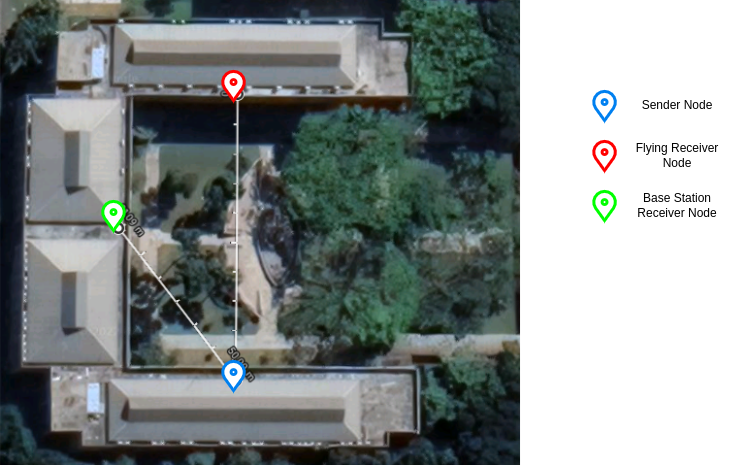
\includegraphics[scale=0.5]{./assets/PetaNonTerbangN}
		\caption{Penempatan node jaringan pada pengujian non-terbang di Gedung N FTE Telkom University.}
	\end{figure}

	\item \textbf{Pengujian terbang - 1 drone - Lapangan BTP}: Pengujian sistem dilakukan dengan menerbangkan \textit{drone} \textit{sender} sejauh 50 meter ke arah selatan dengan ketinggian 10 meter relatif terhadap \textit{remote control}. Node \textit{"flying receiver"} diletakkan di topi penguji untuk menjaga \textit{line-of-sight} dengan node \textit{sender}. Pada pengujian 3 node, maka node \textit{base station} diletakkan di darat, sekitar 20 meter arah selatan dari node \textit{"flying receiver"}.
	\begin{figure}[H]
		\centering
		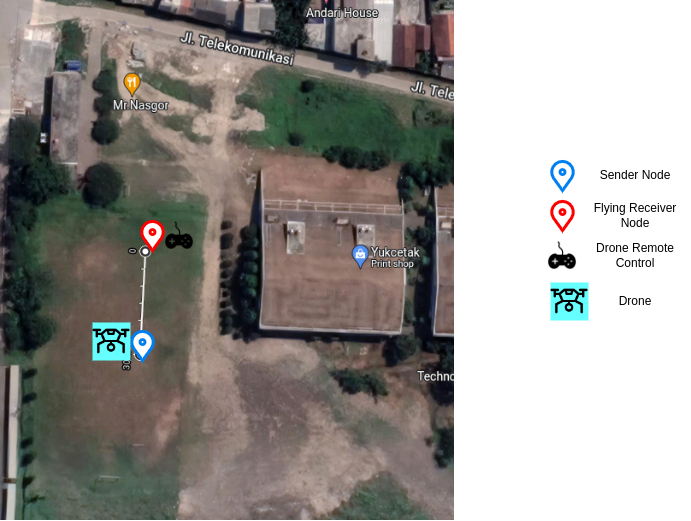
\includegraphics[scale=0.5]{./assets/PetaTerbangSatuBTP}
		\caption{Penempatan node jaringan pada pengujian terbang satu drone di Lapangan BTP Telkom University.}
	\end{figure}

	\item \textbf{Pengujian terbang - 2 drone - Lapangan BTP}: Pengujian sistem 2 drone dilakukan dengan menerbangkan \textit{drone sender} dengan jarak 30 hingga 50 meter terhadap \textit{drone receiver}. Kedua drone ditargetkan mendapatkan ketinggian 10 meter di atas permukaan. Pada pengujian 3 node, maka node \textit{base station} diletakkan di darat, dengan posisi di antara kedua drone.
	\begin{figure}[H]
		\centering
		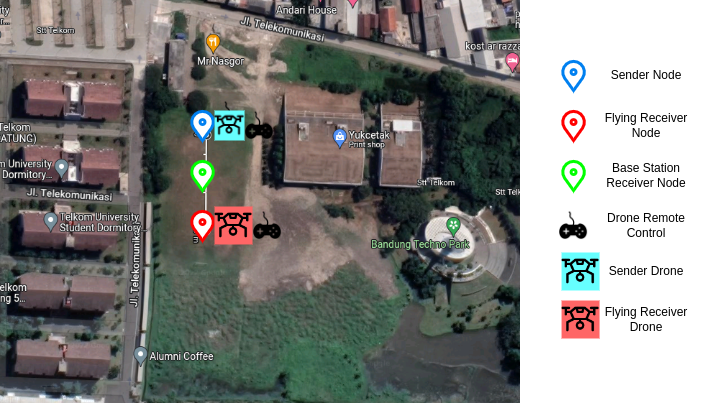
\includegraphics[scale=0.5]{./assets/PetaTerbangDuaBTP}
		\caption{Penempatan node jaringan pada pengujian terbang dua drone di Lapangan BTP Telkom University.}
	\end{figure}

\end{enumerate}

\subsection{Kondisi Lingkungan Pengujian}
Faktor lingkungan dapat mempengaruhi hasil dari pengujian, dengan faktor paling menentukan adalah banyaknya interferensi di pita frekuensi 2.4 GHz terutama dari piranti Wi-Fi di sekitar. Banyaknya interferensi Wi-Fi dapat dilihat menggunakan sebuah program Wi-Fi \textit{Spectrum Analyzer} seperti LinSSID.
\begin{figure}[H]
	\centering
	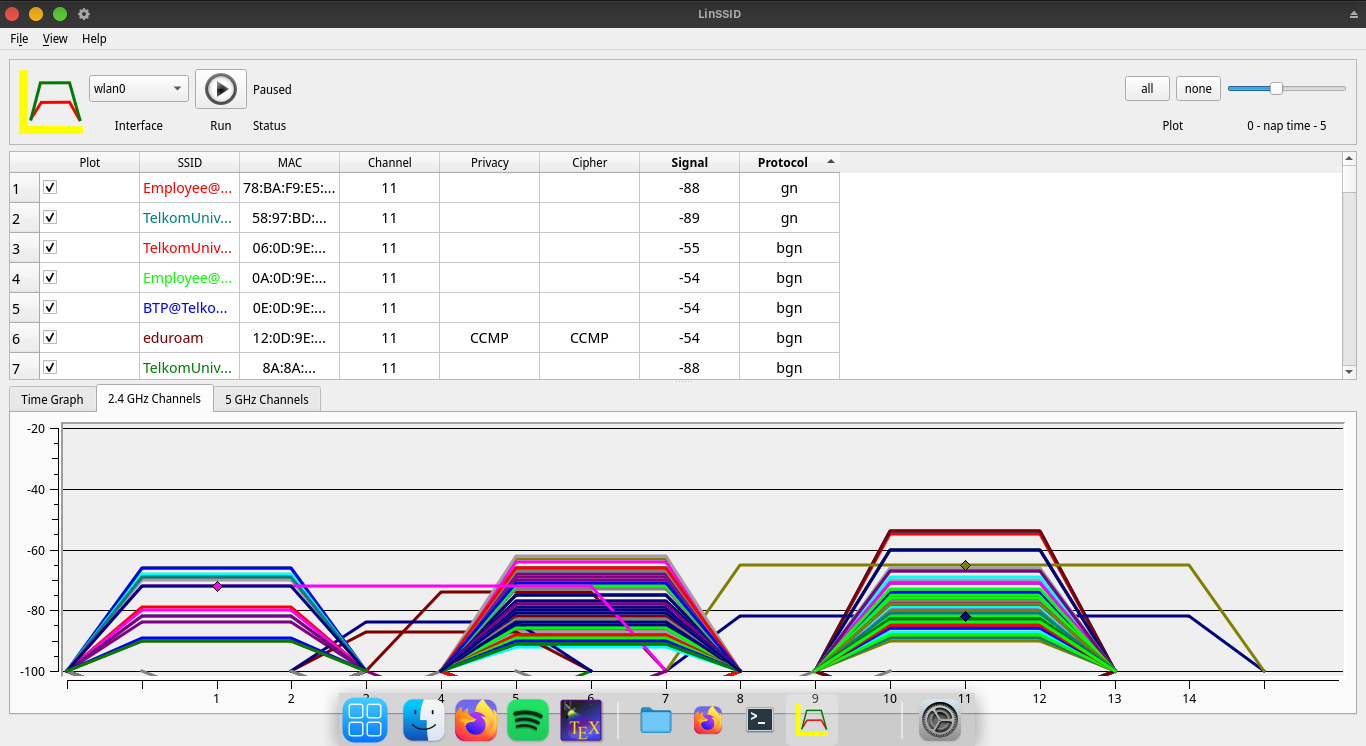
\includegraphics[scale=0.25]{./assets/InterferensiLapanganBTP}
	\caption{Hasil analisis spektrum Wi-Fi 2.4 GHz di Lapangan BTP Telkom University.}
\end{figure}
Gambar 4.4 menunjukkan banyaknya \textit{access point} (AP) Wi-Fi 2.4 GHz di daerah Lapangan BTP Telkom University.
\subsection{Desain Alat}
\subsubsection{Drone \textit{Sender}}
\begin{figure}[H]
	\centering
	\includegraphics[scale=0.1]{./assets/Pengujian/DroneSender}
	\caption{Penampakan implementasi \textit{sender} node di drone MJX Bugs 5W.}
\end{figure}
Drone \textit{sender} merupakan drone yang membawa \textit{board} \textit{sender} node dan dilengkapi dengan kapabilitas GPS. Karena penggunaan drone yang tidak didesain untuk membawa \textit{payload}, maka untuk mengurangi bobot, implementasi \textit{board} ESP32 tidak menggunakan PCB melainkan sepenuhnya menggunakan kabel-kabel \textit{jumper}, serta tidak ada \textit{shroud} pelindung \textit{board}. Antena \textit{omnidirectional} ditempatkan di sisi atas drone untuk menjaga \textit{line-of-sight} terhadap \textit{flying receiver}.
\subsubsection{Drone \textit{Receiver}}

Drone \textit{receiver} merupakan drone yang membawa \textit{board receiver} node dan dilengkapi dengan sebuah \textit{breakout board} MicroSD untuk \textit{logging} data. \textit{Board receiver} menggunakan sebuah \textit{power bank} sebagai sumber daya dan dihubungkan menggunakan kabel USB Micro-B. Pada sistem ini, \textit{board} DOIT-ESP32-DEVKIT dimodifikasi untuk dapat dipasang antena eksternal berbasis SubMiniature-A (SMA) 2.4 GHz, diletakkan di atas \textit{board} dan diposisikan di sisi atas untuk menjaga \textit{line-of-sight} terhadap \textit{sender}.

\subsubsection{\textit{Base Station Receiver}}

Pada node \textit{base station}, sebuah board DOIT-ESP32-DEVKIT dan NodeMCU ESP8266 dipasang di sebuah \textit{breadboard} dan dihubungkan secara UART menggunakan kabel jumper. Pin \verb|VIN| dan \verb|GND| dari masing-masing \textit{board} dihubungkan satu sama lain menggunakan kabel jumper, sehingga kedua \textit{board} dapat dinyalakan secara bersamaan dengan mencolok kabel USB ke salah satu port USB dari kedua \textit{board} tersebut. Pada sistem ini, catu daya yang digunakan adalah sebuah \textit{power bank}.

\section{Skenario Pengujian}
\subsection{Pengujian Tanpa Terbang}

\textbf{DEL JANGAN LUPA MASUKIN GAMBAR PENGUJIAN DISINI}

Pengujian tanpa terbang dilakukan sebanyak dua kali, menguji perbedaan mode Wi-Fi \textit{Long Range} dan Wi-Fi 802.11n. Data yang didapatkan berupa \textit{throughput, round-trip delay} dan \textit{packet loss} komunikasi antara dua node. Karena fungsi \verb|WiFi.RSSI()| pada mikrokontroler ESP32 mengukur kekuatan sinyal antara \textit{station} dengan \textit{access point} dan pada jaringan PainlessMesh terdapat kemungkinan koneksi antara \textit{sender} dan \textit{receiver} tidak terhubung secara langsung melainkan melalui \textit{base station}, maka ada kemungkinan nilai RSSI yang didapatkan pada setiap pengukuran memiliki dua nilai.

Berdasarkan hasil pengukuran dari fungsi \verb|sizeof(msg)|, besar paket data lokasi yang dikirimkan dari \textit{sender} ke \textit{receiver} adalah sebesar 12 byte. Satuan \textit{throughput} yang digunakan adalah Byte per detik (B/s).  Satuan \textit{round-trip delay} yang digunakan \textit{library} PainlessMesh adalah mikrosekon yang kemudian dikonversi menjadi milisekon dengan membagi nilainya dengan 1000. \textit{Packet loss} dihitung setelah 10 kali pengiriman paket penguji \textit{round-trip delay}.

\section{Hasil Pengujian Skenario Komunikasi Dua Drone}
\subsection{Wi-Fi \textit{Long Range}}
\subsection{Wi-Fi 802.11n}

\section{Hasil dan Analisis Hasil Pengujian}
\subsection{Pengujian Tanpa Terbang}
Pengujian tanpa terbang dilakukan di Gedung N FTE Telkom University dengan durasi pengujian 370 detik.
\subsection{Pengujian Terbang Satu Drone}
\subsection{Pengujian Terbang Dua Drone}

\section{Analisis Hasil Pengujian Keseluruhan}